
\documentclass{statsoc}
\usepackage{graphicx}
\usepackage{listings}
\usepackage{color}
\usepackage{amssymb, amsmath, geometry}
\usepackage{natbib}
\usepackage{hyperref}

\makeatletter
\def\maxwidth{\ifdim\Gin@nat@width>\linewidth\linewidth\else\Gin@nat@width\fi}
\def\maxheight{\ifdim\Gin@nat@height>\textheight\textheight\else\Gin@nat@height\fi}
\makeatother
% Scale images if necessary, so that they will not overflow the page
% margins by default, and it is still possible to overwrite the defaults
% using explicit options in \includegraphics[width, height, ...]{}
\setkeys{Gin}{width=\maxwidth,height=\maxheight,keepaspectratio}

\title[STRAIN]{Introducing STRAIN: A simple and interpretable pass rush
metric inspired by materials science}




 
\author[]{Author 1}
\address{Address,
City,
Country}
\email{email1@example.com}

 
\author[]{Author 2}
\address{Address2,
City2,
Country2}
\email{email2@example.com}



% BIBLIOGRAPHY
\usepackage[authoryear]{natbib}
\bibpunct{(}{)}{;}{a}{}{,}


% tightlist command for lists without linebreak
\providecommand{\tightlist}{%
  \setlength{\itemsep}{0pt}\setlength{\parskip}{0pt}}



\usepackage{setspace} \usepackage{booktabs}

\begin{document}


\begin{abstract}
Abstract goes here
\end{abstract}
\keywords{tracking data, Bornn legacy, too much Canadian}

\newpage

\hypertarget{introduction}{%
\section{Introduction}\label{introduction}}

In recent years, tracking data have replaced traditional box-score
statistics and play-by-play data as the state-of-the-art tool in sports
analytics. Numerous sports have been collecting and releasing data on
player and ball locations on the playing surface over the course of a
game. This spatio-temporal multi-resolution source of data have provided
exceptional opportunities for researchers to perform advanced studies at
a more complex level to deepen the understanding of different sports.
For complete surveys on how tracking data have transformed sports
analytics, see \citet{Macdonald2020Recreating}, \citet{Baumer2023Big},
and \citet{Kovalchik2023Player}.

The National Football League (NFL) introduced their player tracking
system known as Next Gen Stats (NGS) in 2016 BDB
\url{https://operations.nfl.com/gameday/technology/nfl-next-gen-stats/}

Previous research bdb this year: linemen Importance of D-linemen, pass
rush (Maybe talk about role of each position, edge vs interior,
defensive formation)

\hypertarget{previous-pass-rush-metrics}{%
\subsection{Previous Pass Rush
Metrics}\label{previous-pass-rush-metrics}}

Limitations

\begin{table}
\caption{A summary of previously-existed pass rush metrics. \label{tab:metrics}}
\centering
\begin{tabular}{ll}
\toprule
\textbf{Metric} & \textbf{Description}\\
\midrule
Sacks & a\\
Hits & a\\
Hurries & a\\
QB Pressures & a\\
Pass-Rush Productivity (PRP) & a\\
Time In Pocket (TIP) & a\\
Pass Rush Win Rate (PRWR) & Rate at which pass rusher beats pass block within 2.5 seconds after snap\\
\bottomrule
\end{tabular}
\end{table}

Table \ref{tab:metrics}

Sacks, hits, hurries, pressures

Officially tracked by the NFL since 1982, the most well known statistic
for evaluating defensive linemen on pass rushing plays is the sack,
which occurs when a defensive player tackles the quarterback behind the
line of scrimmage before the quarterback is able to throw a pass.

\url{https://www.pro-football-reference.com/about/advanced_stats.htm}

Pressures: QB pressures (hurries + knockdowns + sack plays). Note that
``sack plays'' in this instance include both sacks and assists.

Hurried: Times QBs were hurried - defined as a situation when the QB is
forced to throw the ball earlier than intended or is chased around/out
of the pocket as the result of defensive pressure

Hit: Times QBs were hit - occurs when the QB hits the ground after a
throw, not marked on a sack play

PFF's Pass-Rush Productivity (PRP)

\url{https://www.pff.com/news/pro-signature-stats-spotlight-defensive-line}

More recently metrics such as Time In Pocket (TIP) and Pass Rush Win
Rate (PRWR) have also been proposed and are substantial improvements
over the less sophisticated counting statistics.

Pocket Time: Number of seconds the quarterback was in the pocket between
the snap of the ball and a pass or the collapse of the pocket

\citet{Burke2018Created}

\url{https://www.espn.com/nfl/story/_/id/24892208}

2.5 seconds, arbitrary

While PRWR is certainly a step in the right direction, it takes
continuous data and converts it to a binary win/loss, which is generally
not recommended in statistical analysis

\hypertarget{contributions-of-strain}{%
\subsection{Contributions of STRAIN}\label{contributions-of-strain}}

The remainder of this paper is outlined as follows.

\hypertarget{methods}{%
\section{Methods}\label{methods}}

\hypertarget{data}{%
\subsection{Data}\label{data}}

2023 bdb \citep{Howard2023NFL}

first 8 weeks 2021 season

tracking: locations of players and ball, 10 fps,

pre-processing standardize

PFF scouting: pass rush role

sample restriction: remove plays w multiple QB

frames between snap and QB outcome (pass forward, sack)

sample size

\hypertarget{strain-rate-in-materials-science}{%
\subsection{Strain rate in materials
science}\label{strain-rate-in-materials-science}}

\hypertarget{application-to-pass-rushing-in-football}{%
\subsection{Application to pass-rushing in
football}\label{application-to-pass-rushing-in-football}}

\hypertarget{results}{%
\section{Results}\label{results}}

\hypertarget{example-play}{%
\subsection{Example play}\label{example-play}}

\begin{figure}

{\centering 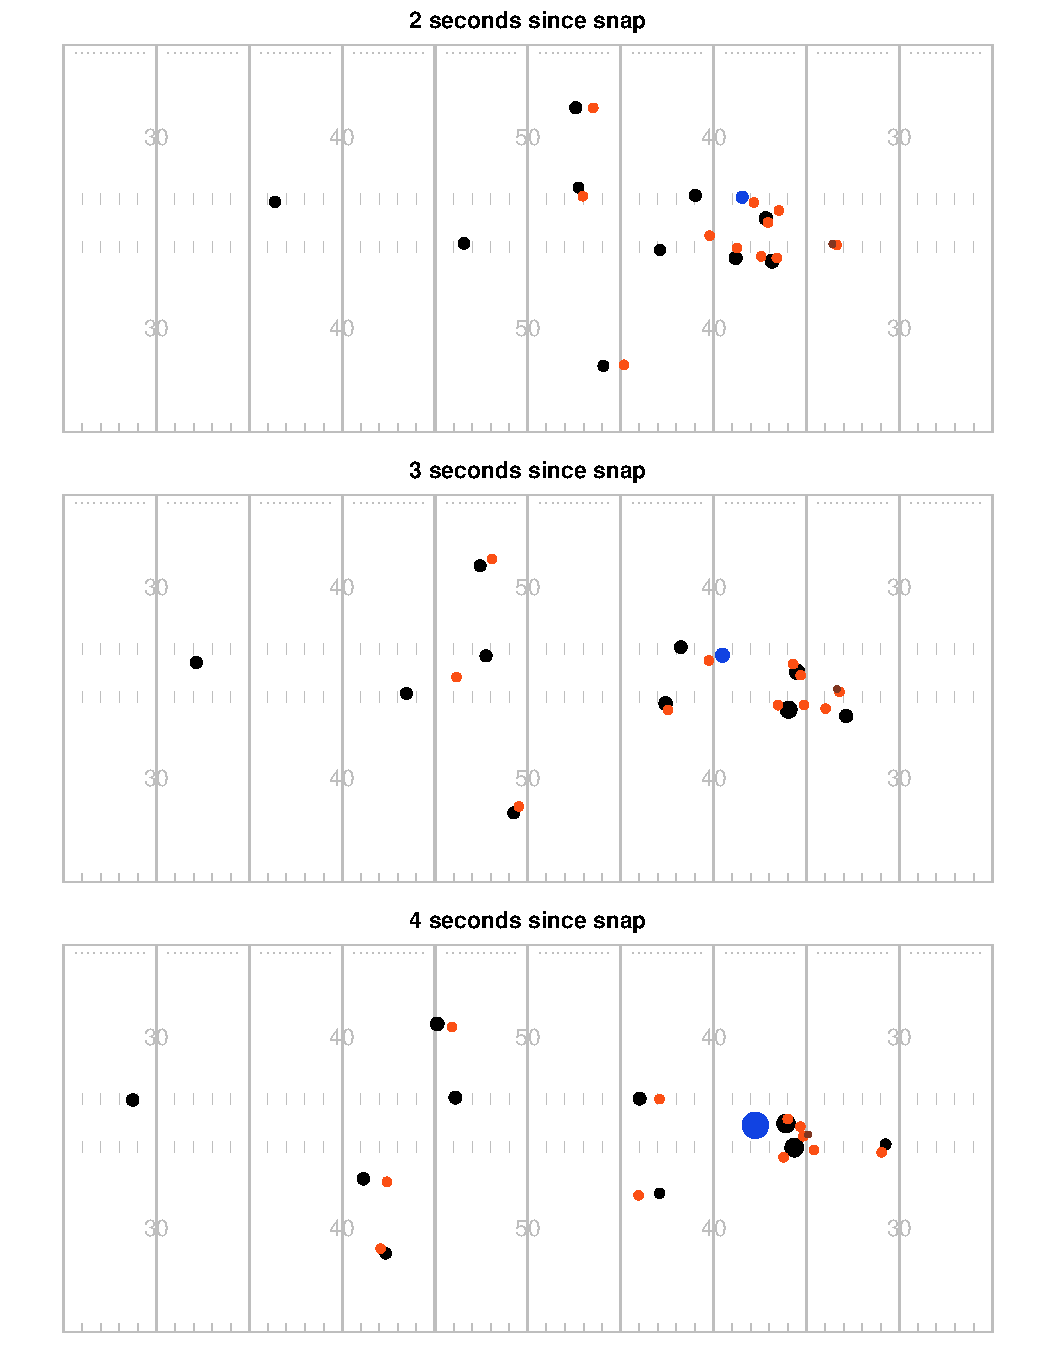
\includegraphics{paper_files/figure-latex/fig_field-1} 

}

\caption{snapshots}\label{fig:fig_field}
\end{figure}

Figure \ref{fig:fig_field} shows snapshots

\begin{figure}

{\centering 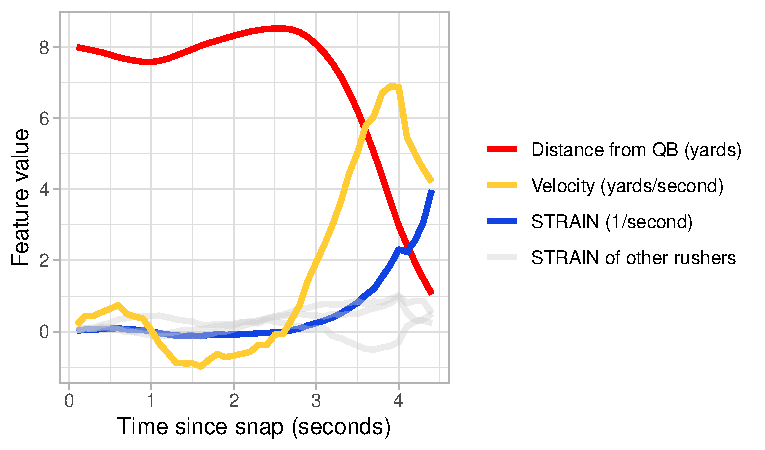
\includegraphics{paper_files/figure-latex/fig_crosby_curves-1} 

}

\caption{crosby}\label{fig:fig_crosby_curves}
\end{figure}

Figure \ref{fig:fig_crosby_curves} shows Crosby throughout the play

\hypertarget{positional-strain-curves}{%
\subsection{Positional STRAIN curves}\label{positional-strain-curves}}

\begin{figure}

{\centering 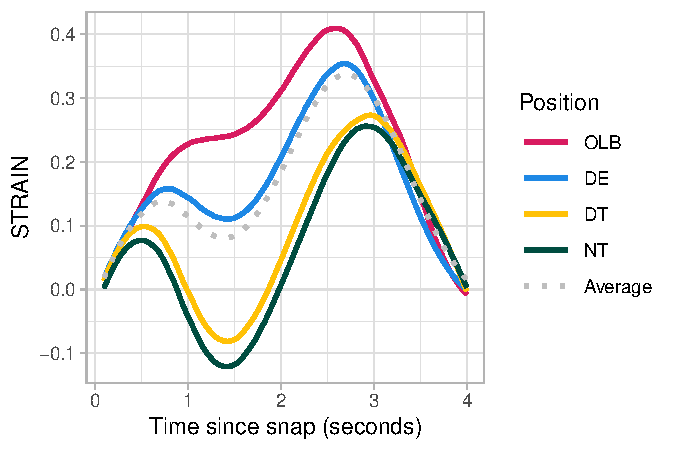
\includegraphics{paper_files/figure-latex/fig_pos_curves-1} 

}

\caption{STRAIN curves for different positions}\label{fig:fig_pos_curves}
\end{figure}

Figure \ref{fig:fig_pos_curves} shows pos curves

\hypertarget{ranking-the-best-pass-rushers}{%
\subsection{Ranking the best
pass-rushers}\label{ranking-the-best-pass-rushers}}

\hypertarget{corr-with-pressure-rate-hits-sacks-hurries-per-snap}{%
\subsection{Corr with pressure rate = (hits + sacks + hurries) per
snap}\label{corr-with-pressure-rate-hits-sacks-hurries-per-snap}}

\begin{figure}

{\centering 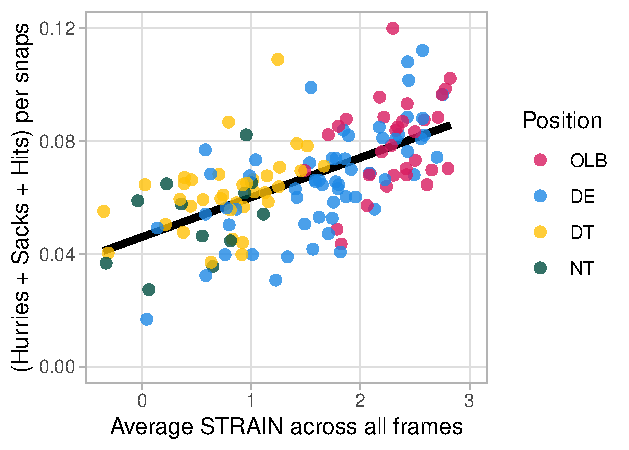
\includegraphics{paper_files/figure-latex/fig_cor_pressure-1} 

}

\caption{Cor with}\label{fig:fig_cor_pressure}
\end{figure}

Figure \ref{fig:fig_cor_pressure} shows cor with pressure

Fairly strong correlation (r = 0.6254943) between average STRAIN \&
hurries + sacks + hits per snaps

\hypertarget{statistical-properties-of-strain}{%
\subsection{Statistical Properties of
STRAIN}\label{statistical-properties-of-strain}}

From \citet{Franks2016Meta} (github
\url{https://github.com/afranks86/meta-analytics})

Discrimination: Does the metric reliably differentiate between players?

Stability: Does the metric measure a quantity which is stable over time?

Independence: Does the metric provide new information?

\begin{figure}

{\centering 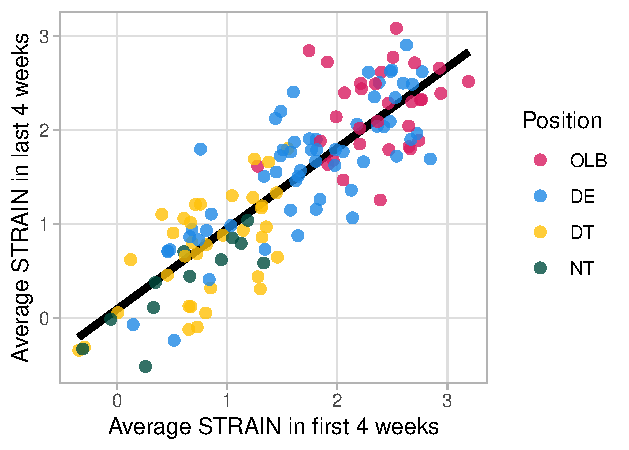
\includegraphics{paper_files/figure-latex/fig_stability-1} 

}

\caption{Metric stability}\label{fig:fig_stability}
\end{figure}

0.8544865

Figure \ref{fig:fig_stability} shows

Average STRAIN across all frames played in first and last 4 weeks

Strong correlation shows great metric stability

\hypertarget{discussion}{%
\section{Discussion}\label{discussion}}

\bibliographystyle{rss}
\bibliography{bibliography}


\end{document}
